\documentclass[a4paper,12pt]{report}
\usepackage[margin=2cm]{geometry}
\usepackage[utf8]{inputenc}
\usepackage{listings} 
\usepackage{graphicx} 
\usepackage{color}
\usepackage{xcolor}
\usepackage{hyperref}
\usepackage{wrapfig}
\usepackage{float}
\usepackage{subcaption}

\newcommand{\currentdata}{ 4 January 2020}

\begin{document}
\vspace{-5cm}
\begin{center}
Department of Computer Science\\
Technical University of Cluj-Napoca\\

\includegraphics[width=10cm]{fig/footer}
\end{center}
\vspace{1cm}
\begin{center}
\begin{Large}
\textbf{Introduction to Artificial Intelligence}\\
\end{Large}
\textit{Laboratory activity 2019-2020}\\
\vspace{3cm}
Project title: Garbage bins placing for maximum demand satisfaction\\
Tool: DEAP\\
\vspace{1.5cm}
Name: Indre Bogdan Marian\\
Group: 30432\\
Email: indremarian@gmail.com\\
\vspace{6cm}
Assoc. Prof. dr. eng. Adrian Groza\\
Adrian.Groza@cs.utcluj.ro\\
\vspace{1cm}

\includegraphics[width=10cm]{fig/footer}
\end{center}

\tableofcontents

\chapter{Getting to know the tool}

The tool used for this project is DEAP (Distributed Evolutionary Algorithms in Python) which is "\textit {novel evolutionary computation framework for rapid prototyping and testing of ideas}" \footnote {Acording to the \href {https://deap.readthedocs.io/en/master/index.html} {official documentation} }. This is a powerfull tool as it offers parallelisation on top of different algorithms and data structures, but for the scoope of this project, parallelisation is not used. 
Instalation of the tool is simple as it comes as a library for python, so a \textbf {pip install deap} will do the trick. Although, there are certain requirements before installation like \textbf {python 2.7, 3.4} or higher, other requirements depend on what it is used for: \textbf {SCOOP} for the computation distribution and \textbf {Numpy} for CMA-ES (Covariance Matrix Adaptation Evolution Strategy). DEAP is developed at the Computer Vision and Systems Laboratory (CVSL) at \href {https://www.ulaval.ca/}{Université Lava}l, in Quebec city, Canada.



\chapter{Running and understanding examples}

DEAP comes with many examples for different purposes. Some of these include:
\begin{enumerate}
\item Genetic Algorithms (GA)
\begin{enumerate}
\item One max problem
\item Knapsack problem
\end{enumerate}
\item Genetic Programming (GP)
\begin{enumerate}
\item Even-Parity Problem
\item Artificial Ant Problem
\end{enumerate}
\item Evolution Strategy (ES)
\begin{enumerate}
\item Evolution Strategies Basics
\item One Fifth Rule
\end{enumerate}
\item Particle Swarm Optimization (PSO)
\begin{enumerate}
\item Particle Swarm Optimization Basics
\item Moving Peaks Benchmark with Multiswarm PSO
\end{enumerate}
\item Estimation of Distributed Algorithms (EDA)
\begin{enumerate}
\item Making Your Own Strategy : A Simple EDA
\end{enumerate}
\end{enumerate}

They all are well explained \href{https://deap.readthedocs.io/en/master/examples/index.html}{here}, but I will focus on GA: One max problem and the classic Knapsack problem.

\section {One Max problem}
One Max offers a simple but efficient problem that can be solved with DEAP and show at the same time the capabilities of the tool. The premise is this: we create a population of integer vectors randomly filled with 0 and 1 then we evolve the population until one of the vectors is full of 1. This example is explained in great detail \href {https://deap.readthedocs.io/en/master/examples/ga_onemax.html}{here}.
\begin{lstlisting}[language=Python]
import random

from deap import base
from deap import creator
from deap import tools

creator.create("FitnessMax", base.Fitness, weights=(1.0,))
creator.create("Individual", list, fitness=creator.FitnessMax)
\end{lstlisting}
An important detail of DEAP is that it does not offer explicit structures, this would be rather impossible. What it offers are tools to create the exact structure is needed. \textbf{Creator} is a class that works as a factory: it can create other classes at run-time, \textbf{Tools} has tools for the evolution and mutation and \textbf{Base} has base classes for evolution algorithms that can be inherited. \textit {creator.create} creates a new class with the name of the first argument, it is inherited from the second and has the attributes of the remaining.  \textit {weights = (1.0,)} creates a tuple with a single argument which means that we want to maximize a single objective.\footnote{For example, weights = (-1.0, 1.0) means that we want to minimize the first objective while maximizing the second)}
\begin{lstlisting}[language=Python]
toolbox = base.Toolbox()
# Attribute generator 
toolbox.register("attr_bool", random.randint, 0, 1)
# Structure initializers
toolbox.register("individual", tools.initRepeat, creator.Individual, 
    toolbox.attr_bool, 100)
toolbox.register("population", tools.initRepeat, list, 
toolbox.individual)
\end{lstlisting}
With the help of the toolbox we can register functions used for generation (attr\_bool) and instantiation (individual, population).
\begin{lstlisting}[language=Python]
def evalOneMax(individual):
    return sum(individual),
\end{lstlisting}
One important feature of genetic algorithms and the place where their "\textit{power}" resides is the evaluation of the individual. That is, in order to reach our goal of a vector filled with 1, we check the sum of the vector. This is the objective we want to maximize.
\begin{lstlisting}[language=Python]
toolbox.register("evaluate", evalOneMax)
toolbox.register("mate", tools.cxTwoPoint)
toolbox.register("mutate", tools.mutFlipBit, indpb=0.05)
toolbox.register("select", tools.selTournament, tournsize=3)
\end{lstlisting}

Next we register the evaluate function, a mate function (in this case a 2 point crossover), a mutation function (flips the bit with the probability of 0.05) and a selection function to select the best individual among a 3 randomly chosen individuals from the population.

\begin{lstlisting}[language=Python]
def main():
    pop = toolbox.population(n=300)
    # Evaluate the entire population
    fitnesses = list(map(toolbox.evaluate, pop))
    for ind, fit in zip(pop, fitnesses):
        ind.fitness.values = fit
    # CXPB  is the probability with which two individuals
    #       are crossed
    #
    # MUTPB is the probability for mutating an individual
    CXPB, MUTPB = 0.5, 0.2
\end{lstlisting}

Here we are creating the population (of 300 individuals) and we evaluate it by applying the evaluation function on each individual from the pop. This fitness is attributed to each individual.

\begin{lstlisting}[language=Python]
# Extracting all the fitnesses of 
    fits = [ind.fitness.values[0] for ind in pop]
    # Variable keeping track of the number of generations
    g = 0
    
    # Begin the evolution
    while max(fits) < 100 and g < 1000:
        # A new generation
        g = g + 1
        print("-- Generation %i --" % g)
        # Select the next generation individuals
        offspring = toolbox.select(pop, len(pop))
        # Clone the selected individuals
        offspring = list(map(toolbox.clone, offspring))
        # Apply crossover and mutation on the offspring
        for child1, child2 in zip(offspring[::2], offspring[1::2]):
            if random.random() < CXPB:
                toolbox.mate(child1, child2)
                del child1.fitness.values
                del child2.fitness.values
        for mutant in offspring:
            if random.random() < MUTPB:
                toolbox.mutate(mutant)
                del mutant.fitness.values
        # Evaluate the individuals with an invalid fitness
        invalid_ind = [ind for ind in offspring if not ind.fitness.valid]
        fitnesses = map(toolbox.evaluate, invalid_ind)
        for ind, fit in zip(invalid_ind, fitnesses):
            ind.fitness.values = fit
        pop[:] = offspring
\end{lstlisting}

As the evolution begins, we must keep track of the generations that pass while also following the fitness of the individuals to know when to stop (100 means we have an individual filled with 1). Next steps are to clone the best individuals and to mate and mutate them to obtain better individuals, this also means that some individuals loose their original fitness and we must reassess it. lastly, we copy the offsprings to the population.

\begin{lstlisting}[language=Python]
# Gather all the fitnesses in one list and print the stats
        fits = [ind.fitness.values[0] for ind in pop]
        
        length = len(pop)
        mean = sum(fits) / length
        sum2 = sum(x*x for x in fits)
        std = abs(sum2 / length - mean**2)**0.5
        
        print("  Min %s" % min(fits))
        print("  Max %s" % max(fits))
        print("  Avg %s" % mean)
        print("  Std %s" % std)
\end{lstlisting}

An additional step is the printing of some stats as the evolution progresses. After it is run, here are the results:
\begin{lstlisting}
Start of evolution
  Evaluated 300 individuals
-- Generation 1 --
  Evaluated 181 individuals
  Min 44.0
  Max 66.0
  Avg 54.833333333333336
  Std 4.349584909952722
-- Generation 2 --
  Evaluated 191 individuals
  Min 47.0
  Max 68.0
  Avg 58.45666666666666
  Std 3.455641120769904
-- Generation 3 --
  Evaluated 199 individuals
  Min 52.0
  Max 68.0
  Avg 60.95333333333333
  Std 2.9024970092816367
...
...
...
-- Generation 34 --
  Evaluated 182 individuals
  Min 88.0
  Max 99.0
  Avg 96.77333333333333
  Std 2.0917191228485437
-- Generation 35 --
  Evaluated 177 individuals
  Min 86.0
  Max 100.0
  Avg 97.04333333333334
  Std 2.325536975028139
-- End of (successful) evolution --
Best individual is [1, 1, 1, 1, 1, 1, 1, ... 1, 1, 1, 1], (100.0,)
\end{lstlisting}

This means that in 35 generations we have reached our goal. We can also see the constant improvement in stats: from an average of 54 in the first generation, to one of 97 in the last. Small changes in the mutation or crossover coefficient can create create scenarios where we find very hard the right answer, if we find it at all! 

\begin{enumerate}
\item For a mutation of 0.7
\begin{lstlisting}
-- Generation 510 --
  Evaluated 256 individuals
  Min 79.0
  Max 100.0
  Avg 89.74666666666667
  Std 3.339035123438477
-- End of (successful) evolution --
\end{lstlisting}

\item For a crossovern of 0.1

\begin{lstlisting}
-- Generation 127 --
  Evaluated 86 individuals
  Min 88.0
  Max 100.0
  Avg 97.90666666666667
  Std 2.2857432537846467
-- End of (successful) evolution --
\end{lstlisting}
\end{enumerate}

\section {Knapsack problem}

The Knapsack problem is a classic problem of optimization. Here we have to fill the knapsack with the most valuable items while minimizing the total weight. Only the important changes from the previous problem wil be shown.

\begin{lstlisting}[language=Python]
creator.create("Fitness", base.Fitness, weights=(-1.0, 1.0))
creator.create("Individual", set, fitness=creator.Fitness)
# Create the item dictionary: item name is an integer, and value is 
# a (weight, value) 2-uple.
items = {}
# Create random items and store them in the items' dictionary.
for i in range(NBR_ITEMS):
    items[i] = (random.randint(1, 10), random.uniform(0, 100))
\end{lstlisting}

One difference is the fact that here we use a set as it is closer to reallity (we will be dealing with the 0-1 Knapsack problem) and we take into account both the weight and the value when we create the fitness.

\begin{lstlisting}[language=Python]
def evalKnapsack(individual):
    weight = 0.0
    value = 0.0
    for item in individual:
        weight += items[item][0]
        value += items[item][1]
    if len(individual) > MAX_ITEM or weight > MAX_WEIGHT:
        return 10000, 0             # Ensure overweighted bags are dominated
    return weight, value
def cxSet(ind1, ind2):
    """Apply a crossover operation on input sets. The first child is the
    intersection of the two sets, the second child is the difference of the
    two sets.
    """
    temp = set(ind1)                # Used in order to keep type
    ind1 &= ind2                    # Intersection (inplace)
    ind2 ^= temp                    # Symmetric Difference (inplace)
    return ind1, ind2
def mutSet(individual):
    """Mutation that pops or add an element."""
    if random.random() < 0.5:
        if len(individual) > 0:     # We cannot pop from an empty set
            individual.remove(random.choice(sorted(tuple(individual))))
    else:
        individual.add(random.randrange(NBR_ITEMS))
    return individual,
\end{lstlisting}

Another change is the fact that a new evaluation function is needed, but an interesting thing is the need for a new crossover and mutation functions. This is because there are no such functions offered by DEAP on sets so they must be made manually. Here are the results:

\begin{lstlisting}
gen	nevals             min                      	max                        
0  	50    	[10.         49.69958685]	[ 38.         345.35491309]
1  	87    	[0. 0.]                  	[ 45.         414.48478381]
2  	91    	[0. 0.]                  	[ 28.         414.48478381]
...
...
48 	86    	[0. 0.]                  	[ 47.         707.73092646]
49 	90    	[0. 0.]                  	[ 47.         707.73092646]
50 	87    	[0. 0.]                  	[ 47.         707.73092646]
\end{lstlisting}

As can be seen, the best individual after 50 generations is with a weight of 47 and a value of 707.

\chapter{Project description}

\section {Project narative}
Waste disposal in cities has always been a challenge for public administrators and city planners\cite{purkayastha2015pollution}. Long gone are the days when disposal was simply done in rivers and other bodies of water, we have evolved, but so did our cities. Now there is a need for complex and efficient solutions to manage our garbage and reduce both the costs and the pollution of the enviroment.
This project is meant as a small solution to a small but complex problem in this field. Using GAs I decided to give a helping hand to the people that take care of placing garbage bins in an area.
Let us have a look at a possible scenario in the real world. The council of a city has just been given a certain budged to spend on new smart bins to replace the old garbage bins around the city. There are many decisions that come into play here, some of which demand that:
\begin{enumerate}
\item The bins should cover as much area as possible and should be placed in this way
\item The bins should cover as much of the waste demand \footnote{Waste Demand refers to the amount of garbage a certain place is creating} as possible
\end{enumerate}
By having historical data on how much garbage certain buildings and places output, this project will provide the best places for the smart bins and also the volume they should have in order to satisfy the garbage demand.

\section {Facts and Specifications}
Firstly, data about the amount of waste produced by an area \footnote{Areas can be buildings, public places neighbourhoods etc} must be given. These areas will provide an insight into the what exactly is needed but they are not enough.
Both in recycling and waste disposal, distance plays a big factor\cite{castro2017smart} so the distance from one area to the smart bin is measured in other areas (1-2) away. People are creatures of habbit and they will dump their garbage usually in the same place, and usually to the closest place available. I have considered that all the people in an area will dump their garbage in the that area if a bin is present, 50\% of people will come from an area away and only 25\% will come from 2 areas away. Those percentages can be adjusted as specialists see fit.
Secondly, depending on the size of the map, the amount of waste produced and the number of bins we have at our disposal we miht not be able to fully cover the map. In this case we can still find out what coverage we have and estimate how many more bins we need.

\section {Top level design}
The system must get the historical data and read it in a matrix. This will be used to create our individuals and population. The individuals are considered to be integer vectors of double the number of input bins. Each pair of numbers from the vector represent the coordinates of a bin in the matrix. An evaluation function that maximizes coverage and keeps the minimum size of the bin in that area will be needed. We must make sure as we mutate and make crossovers that we remain in the map so a decorator is required.
Further development could be done to make the system more computationally efficient and to make it more specific for the bin size and maybe even compute the best option based on a budged.

\chapter{Implementation}
\section {Setup}
In order to create an evolution, we need certain things which are common to all GAs: a representation of an individual, the creation of a population, the crossover and mutation of that population, a way to evaluate the fitness of the individuals and a way of selecting the best individuals to become the new population. This process is reaped until a goal is reached or until a number of generations have past. Fortunatelly, DEAP makes all of this very easy and short with the \textbf{creator} and \textbf{toolbox}. As shown in the examples, few things must be changed in order to have a framework for the algorithm.
\begin{lstlisting}[language=Python]
creator.create("FitnessMax", base.Fitness, weights=(1.0,))
creator.create("Individual", list, fitness=creator.FitnessMax)
\end{lstlisting}

One important thing to take care of is the fitness. Here we want to maximize the coverage

\begin{lstlisting}[language=Python]
toolbox.register("attr_pos", random.randint, 0, max(matrix.shape)-1)
toolbox.register("individual", tools.initRepeat, creator.Individual, 
    toolbox.attr_pos, settings.individualLength)
toolbox.register("population", tools.initRepeat, list, toolbox.individual)
\end{lstlisting}

The individual is represented by the position atributte that is a random integer from 0 to the maximum size of the matrix (map).

\begin{lstlisting}[language=Python]
toolbox.register("mate", tools.cxTwoPoint)
toolbox.register("mutate", tools.mutUniformInt, low=0, up=max(matrix.shape), indpb=0.05)
toolbox.register("select", tools.selTournament, tournsize=3)
\end{lstlisting}

The mate, mutate and selection function are chosen. Although DEAP offers many types of crossovers (One point crossover, partially matched crossver, ordered crossover, blend crossover etc), mutation ( Gaussian mutation, shuffle mutation, polynomial mutation etc), I have chosen a simple but effcient Two Point crossover and a Uniform mutation.
Lastly we have the actual evolution which can be summed up with the schema on the next page.
\begin{figure}[H]
    \centering
    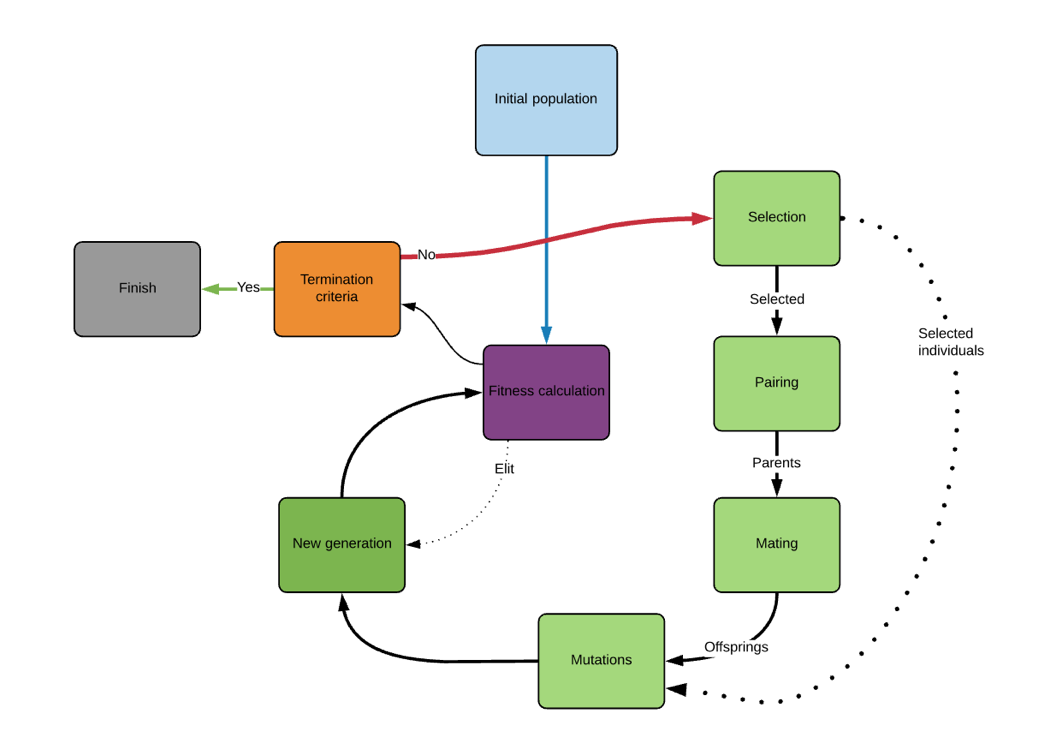
\includegraphics[width=1\textwidth]{fig/schema}
    \caption{GA flow ..... }
%\href{https://towardsdatascience.com/continuous-genetic-algorithm-from-scratch-with-python-ff29deedd099}{https://towardsdatascience.com/continuous-genetic-algorithm-from-scratch-with-python-ff29deedd099}}
    \label{fig:schema}
\end{figure}


\section{The evaluation function}
The power of Genetic Algorithms resides in the evaluation function. This means that in order to have an efficient GA where we reach the optimization levels we want, we need a good evaluation of the individual. For this project I started small and incremented this function with small adjustments.

\begin{lstlisting}[language=Python]
def evalSurfaceCovered(individual):
    
    matrixBool = np.full(matrix.shape, 0)
    surface = 0
    
    for t in range(0, settings.individualLength-1, 2):
        if matrixBool.item(individual[t], individual[t+1]) == 0 :
            surface += matrix.item(individual[t], individual[t+1])
            matrixBool[individual[t], individual[t+1]] = 1
    return surface,
\end{lstlisting}

This is the first version of the function. Here I just find the maximum coverage of one area

\begin{lstlisting}[language=Python]
def evalSurfaceCoveredMatrix(individual):
    
    matrixBool = np.full(matrix.shape, 0)
    surface = 0
    
    for t in range(0, settings.individualLength - 1, 2):
        if matrixBool.item(individual[t], individual[t+1]) == 0 :
            for i1 in range(-1,2):
                for i2 in range(-1,2):
                        try:
                            if matrixBool.item(individual[t] + i1,
		          		 individual[t+1] + i2) == 0 :
                                surface += matrix.item(individual[t] + 
                              		  i1, individual[t+1] + i2)
                                matrixBool[individual[t] + i1, 
                               		 individual[t+1] + i2] = 1
                        except IndexError:
                            continue 
    return surface,
\end{lstlisting}

In this version I consider a full matrix of 9 areas (so a 1 tile influence), but it does not take into consideration the percentages and consideres that 100\% of the people in the areas next to the bin area will go to this bin.

\begin{lstlisting}[language=Python]
def evalSurfaceCoveredMatrixVar(individual):
    
    matrixBool = np.full(matrix.shape, 0)
    surface = 0
    
    for t in range(0, settings.individualLength - 1, 2):
        try:
            if matrixBool.item(individual[t], individual[t+1]) == 0 :
                for i1 in range(-1,2):
                    for i2 in range(-1,2):
                            try:
                                if (individual[t] + i1) < 0 or
				 (individual[t+1]+ i2) < 0:
                                    raise IndexError
                                if matrixBool.item(individual[t] + i1,
					 individual[t+1] + i2) == 0 :
                                    surface += matrix.item(individual[t] +
						i1, individual[t+1] + i2)
                                    matrixBool[individual[t] + i1,
						 individual[t+1] + i2] = 1
                            except IndexError:
                                continue 
        except IndexError:
            return 0, 
    return surface,
\end{lstlisting}

Here I took into consideration the shape of the map (now it can be rectangunlar and it will not give any error).

\begin{lstlisting}[language=Python]
def evalSurfaceCoveredMatrixVarDisperse(individual):
    #print(individual)
    matrixCopy = copy(matrix)
    surface = 0
    volume = 0
    
    for t in range(0, settings.individualLength - 1, 2):
        for i1 in range(-2,3):
            for i2 in range(-2,3):
                    try:
                        if (individual[t] + i1) < 0 or
			 (individual[t+1] + i2) < 0:
                            raise IndexError
                        TileCopy = matrixCopy.item(
				individual[t] + i1, individual[t+1] + i2)
                        TileOriginal = matrix.item(
				individual[t] + i1, individual[t+1] + i2)
                        
                        if i1 == 0 and i2 == 0:
                            volume = (settings.volumeCenter * 
						TileOriginal) / 100
                        else:
                            if i1 > 1 or i1 < -1 or i2 > 1 or i2 < -1:
                                volume = (settings.volumeTwoTilesAway
						* TileOriginal) / 100
                            else:
                                volume = (settings.volumeOneTileAway 
						* TileOriginal) / 100
                        
                        if TileCopy > 0:       
                            if volume > TileCopy:
                                surface +=  TileCopy
                            else:
                                surface += volume
                        
                        matrixCopy[individual[t] + i1,
				 individual[t+1] + i2] -= volume
                    except IndexError:
                        continue 
    
    return surface * 100 / maxDemand,
\end{lstlisting}

Lastly, the final version. Here I changed the criteria to find the maximum demand (in percentage) and I put into practice the influence system. 100\% from the area of the bin, 50\% from the next areas and 25\% from the next.

\section {Bounds check}
This is the final addition that is needed in order to avoid bad individuals.

\begin{lstlisting}[language=Python]
def checkBounds():
    def decorator(func):
        def wrapper(*args, **kargs):
            offspring = func(*args, **kargs)
            for child in offspring:
                for i in range(0, len(child)-1, 2):
                    if child[i] > matrix.shape[0] - 1:
                        child[i] = random.randint(0,
				matrix.shape[0] - 1)
                    if child[i+1] > matrix.shape[1] - 1:
                        child[i+1] = random.randint(0,
				 matrix.shape[1] - 1) 
            return offspring
        return wrapper
    return decorator

toolbox.decorate("mate", checkBounds())
toolbox.decorate("mutate", checkBounds())
toolbox.decorate("population", checkBounds())
\end{lstlisting}

This is a decorator that we apply on mating, mutation and the initial population.

\chapter{Results}

The results of the system depend on the input map, influence percentages, the number of bins we want to create but also on the crossover and mutation coefficients.
\section {An example}

\begin{lstlisting}
1 1 1 1 1 1 1 1 1 1
1 1 1 1 1 1 1 1 1 1
1 10 1 1 1 1 1 1 1 1
1 1 1 1 1 10 1 1 1 1
1 1 1 1 1 1 1 1 1 1
1 1 1 1 1 1 1 1 1 1
1 1 1 1 1 1 1 1 1 1
1 10 1 1 1 1 1 1 1 10
1 1 1 1 1 1 1 1 1 1
1 1 1 1 1 1 1 1 1 1
1 1 1 1 1 1 1 1 1 1
1 1 1 1 1 1 1 1 1 1
1 1 1 1 1 1 1 1 1 1
1 1 1 1 1 1 1 1 1 1
1 1 1 1 1 1 1 1 1 1
1 1 1 1 1 1 1 1 1 1
1 1 1 1 1 1 1 1 1 1
1 1 1 1 1 1 1 1 1 1
\end{lstlisting}
We consider this to be the average historical volume of garbage during a period of time. Below we have the other settings.

\begin{lstlisting}[language=Python]
self.nrOfBins = 38
self.volumeCenter = 100
self.volumeOneTileAway = 50
self.volumeTwoTilesAway = 25
self.CXPB = 0.5
self.MUTPB = 0.2
\end{lstlisting}

For this specific input, these are the results of the first generation

\begin{figure}[H]
    \centering
    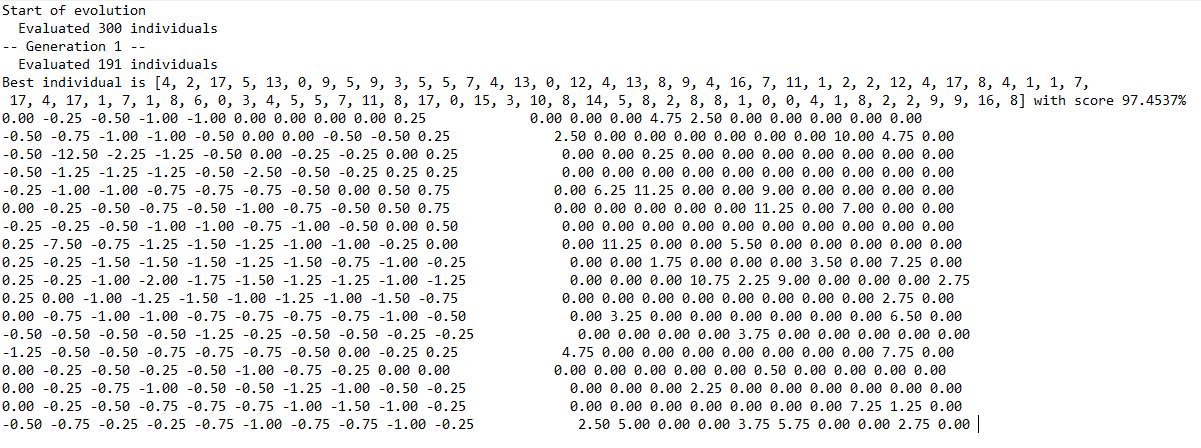
\includegraphics[width=1\textwidth]{fig/results1}
    \caption{First Generation with best individual}
    \label{fig:results1}
\end{figure}

As specified above, the position of the bins are represented by the integers in the individual, every pair of integers is the coordinates of a bin.

\begin{figure}[H]
    \centering
    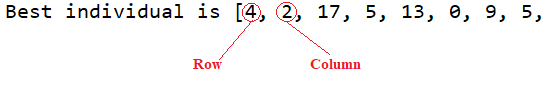
\includegraphics[width=1\textwidth]{fig/best1}
    \caption{Best individual}
    \label{fig:best1}
\end{figure}

\begin{figure}[H]
    \centering
    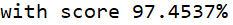
\includegraphics[width=0.5\textwidth]{fig/score}
    \caption{The score of the best individual}
    \label{fig:score}
\end{figure}
\begin{figure}[H]
    \centering
    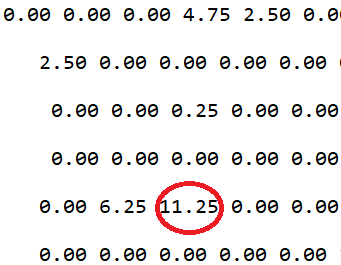
\includegraphics[width=0.5\textwidth]{fig/position1}
    \caption{The position of the Bin on the map}
    \label{fig:position1}
\end{figure}

The system not only shows the position but it also provides information on what is the minimum volume that bin must have in order to satisfy the demand around. Every 0 represents an area where no bin was placed and everything greater than 0 is the minimum volume.

\begin{figure}[H]
    \centering
    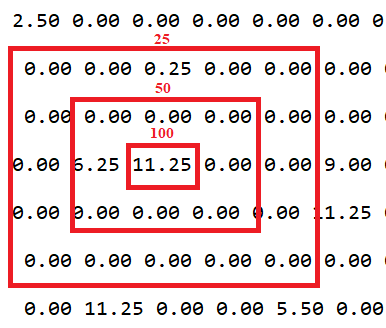
\includegraphics[width=0.5\textwidth]{fig/influence1}
    \caption{The influence of the bin}
    \label{fig:influence1}
\end{figure}

This shows the percentage of the volume the people in the respective areas will bring to the bin.

\begin{figure}[H]
    \centering
    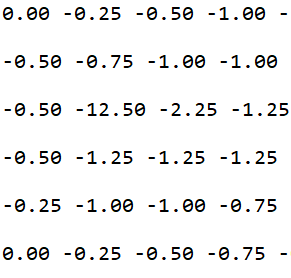
\includegraphics[width=0.5\textwidth]{fig/remaining}
    \caption{Remaining and surplus demand}
    \label{fig:remaining}
\end{figure}
On the left matrix, we have the remaining demand (positive numbers) and the surplus demand (what we can add in terms of waste and the system still remains valid).
For this example, 33 generations were needed to find a score of 100\%. This is the best overall individual.
\begin{figure}[H]
    \centering
    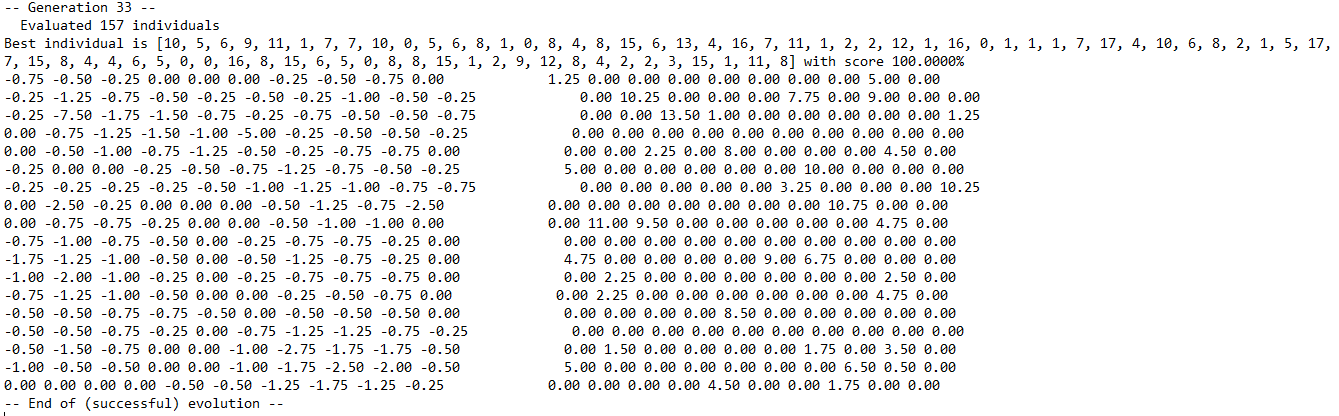
\includegraphics[width=1\textwidth]{fig/results3}
    \caption{Final result}
    \label{fig:results3}
\end{figure}

To better understand the results, some statistics should be computed. For simplicity, the minimum, maximum, mean and standard deviation of the fitness has been computed.

\begin{figure}[H]
 \centering
\begin{subfigure}{0.3\textwidth}
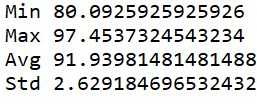
\includegraphics[width=0.9\linewidth]{fig/stats1} 
\caption{First generation}
\label{fig:stats1}
\end{subfigure}
\begin{subfigure}{0.3\textwidth}
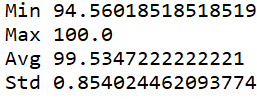
\includegraphics[width=0.9\linewidth]{fig/stats2}
\caption{Last generation}
\label{fig:stats2}
\end{subfigure}
 
\caption{Evolution statistics}
\label{fig:ev}
\end{figure}

The mean (Avg) is computed as 
 \[ \bar{x} = \sum {\frac{x_i}{n}} \]
And the standard deviation (Std) as
\[ s = \sqrt{\frac{\sum_{i=1}^n(x_i - \bar{x}^2)}{n-1}}  \]
Here we can see the evolution of population which shows that the average fitness is growing steadly but it also shows it's convergence because of the decreasing standard deviation.

\section {Future development}
There are many possible improvements that can be added, some examples include: 
\begin{enumerate}
\item a better evaluation function
\item inclusion of the volume found in the individual
\item refactoring of the code
\item a better representation of the map
\item completing the system: not only finding the places for the bins, but also using GAs to schedule the dump trucks to reduce costs and finding the best routes by taking into account how full the bins are
\item etc.
\end{enumerate}
\chapter{Conclusion}
While this paper tries and does find a solution to the existing problem, there is no hiding from the fact that better solution already exist, solutions that use different methods and have more accurate results\cite{sumedh2015gis}. This work is meant as an exploration and application of Genetic Algorithms into the public administration domain. From this perspective it, I do believe that I have learned a lot and it has improved my reasearch skills greatly.

\appendix

\chapter{Your original code}
\label{app:code}
This section should contain only code developed by you, without any line re-used from other sources. 
This section helps me to correctly evaluate your amount of work and results obtained. 
Including in this section any line of code taken from someone else leads to failure of IS class this year.
Failing or forgetting to add your code in this appendix leads to grade 1.
Don't remove the above lines.\\
\textbf{Observation}
I have not added here the setup, the evolution and the bounds check as they have been changed from other pieces of code\cite{doc} to suit the need of this project. The setup and the bounds check can be found in the implementation chapter, the evolution is similar to the one from the One Max Problem in chapter 2.
\begin{lstlisting}[language=Python]
class Settings():
    """A class to store the settings"""
    
    def __init__(self):
        """Initializes static settings"""
        self.nrOfBins = 38
        self.individualLength = 2 * self.nrOfBins
        self.volumeCenter = 100
        self.volumeOneTileAway = 50
        self.volumeTwoTilesAway = 25
        self.CXPB = 0.5
        self.MUTPB = 0.2


def read_matrix():
    with  open("city/matrix.txt") as matrixFile:
        resultList = []
        for line in matrixFile:
            line = line.rstrip('\n')
            sVals = line.split(" ")
            iVals = list(map(np.float, sVals))
            resultList.append(iVals)
        matrixFile.close()
    return np.asmatrix(resultList)

matrix = read_matrix()
maxDemand = matrix.sum()
settings = Settings()

def evalSurfaceCoveredMatrixVarDisperse(individual):
    #print(individual)
    matrixCopy = copy(matrix)
    surface = 0
    volume = 0
    
    for t in range(0, settings.individualLength - 1, 2):
        for i1 in range(-2,3):
            for i2 in range(-2,3):
                    try:
                        if (individual[t] + i1) < 0 or
				 (individual[t+1] + i2) < 0:
                            raise IndexError
                        TileCopy = matrixCopy.item(
				individual[t] + i1, individual[t+1] + i2)
                        TileOriginal = matrix.item(
				individual[t] + i1, individual[t+1] + i2)
                        
                        if i1 == 0 and i2 == 0:
                            volume = (settings.volumeCenter * 
						TileOriginal) / 100
                        else:
                            if i1 > 1 or i1 < -1 or i2 > 1 or i2 < -1:
                                volume = (settings.volumeTwoTilesAway 
						* TileOriginal) / 100
                            else:
                                volume = (settings.volumeOneTileAway 
						* TileOriginal) / 100
                        
                        if TileCopy > 0:       
                            if volume > TileCopy:
                                surface +=  TileCopy
                            else:
                                surface += volume
                        
                        matrixCopy[individual[t] + i1,
				 individual[t+1] + i2] -= volume
                    except IndexError:
                        continue 
    
    return surface * 100 / maxDemand,

def showBestIndividual(individual):
    matrixCopy = copy(matrix)
    matrixVolume = np.full(matrix.shape, 0, dtype=float)
    volume = 0
    
    for t in range(0, settings.individualLength - 1, 2):
        individualVolume = 0
        for i1 in range(-2,3):
            for i2 in range(-2,3):
                try:
                    if (individual[t] + i1) < 0 or 
				(individual[t+1] + i2) < 0:
                        raise IndexError
                    TileCopy = matrixCopy.item(
			individual[t] + i1, individual[t+1] + i2)
                    TileOriginal = matrix.item(
			individual[t] + i1, individual[t+1] + i2)
                        
                    if i1 == 0 and i2 == 0:
                        volume = (settings.volumeCenter 
				* TileOriginal) / 100
                    else:
                        if i1 > 1 or i1 < -1 or i2 > 1 or i2 < -1:
                            volume = (settings.volumeTwoTilesAway 
				* TileOriginal) / 100
                        else:
                            volume = (settings.volumeOneTileAway 
				* TileOriginal) / 100
                        
                    if TileCopy > 0:       
                        if volume > TileCopy:
                            individualVolume +=  TileCopy
                        else:
                            individualVolume += volume
                    matrixCopy[individual[t] + i1,
			 individual[t+1] + i2] -= volume
                except IndexError:
                    continue 
        matrixVolume[individual[t],
			 individual[t+1]]= individualVolume
    
    for i in range(0, matrix.shape[0]):
        for j in range(0, matrix.shape[1]):
            print("\%.2f " \% matrixCopy[i][j], end='')
        print("            ", end='')
        for j in range(0, matrix.shape[1]):
            print("\%.2f " \% matrixVolume[i][j], end='')
        print()
       
\end{lstlisting}

\bibliographystyle{plain}
\bibliography{ai}


\vspace{2cm}
\begin{center}

\includegraphics[width=10cm]{fig/footer}
\end{center}



\end{document}
